% Rafael Sartori M. dos Santos, 186154
\documentclass[brazilian,a4paper,twocolumn]{article}

% Título
\title{MC920 -- Trabalho 1}
\author{Rafael Sartori M. Santos, 186154}
\date{11 de setembro de 2019}

% Configuração do documento
\setlength{\parskip}{3pt}
\usepackage[utf8]{inputenc} % tipo de documento UTF-8
\usepackage{mathtools} % permitir expressões matemáticas
\usepackage{babel} % configuração da lingua portuguesa
\usepackage{caption} % para legenda de tabelas e figuras
\usepackage[
    pdfauthor={Rafael Sartori M. Santos},
    pdftitle={Trabalho 1 -- MC920},
    pdfproducer={LaTeX (texlive) com hyperref}
]{hyperref} % para links externos (href)
\usepackage{cleveref} % para referenciar tabelas e figuras melhor
\usepackage{indentfirst} % indentação de todo primeiro parágrafo
\usepackage{graphicx} % para adicionar imagens
\usepackage{subcaption} % para imagens ficarem lado a lado
% Usamos geometry pois dá mais espaço que fullpage
%\usepackage{geometry} % alterar geometria do papel
%\geometry{a4paper,left=1.7cm,right=1.7cm,top=1cm,bottom=2.0cm} % menor margem
\usepackage{fullpage} % utilizamos uma versão com menos espaçamento nas bordas

% Início do documento
\begin{document}

\maketitle

\section{Introdução}

    O objetivo do trabalho é analisar, no processo de \textit{half-toning}, os diferentes métodos de difusão de erro: Floyd-Steinberg, Sevenson-Arce, Burkes, Sierra, Stucki e Jarvis-Judice-Ninke. Aplicarei uma transformação em 2 níveis para cada camada de cor de uma imagem representada com 3 camadas: vermelho, verde e azul (R, G, B). Obteremos ao final $8$ possibilidades de cor para cada ponto da imagem. Analisarei uma imagem de grande dimensão no formato PNG quanto a sua semelhança à original em uma tela de computador em 2 casos: curta e longa distância de visualização.

    Farei esse processamento utilizando Python com as bibliotecas \href{https://opencv.org/}{\emph{OpenCV}} e \href{https://numpy.org/}{\emph{NumPy}} em um \href{https://jupyter.org/}{\emph{Jupyter Notebook}}.


\section{Método}

    Capturei uma imagem de grande dimensão (3096x4128) colorida com meu celular sob condições de alta luminosidade, pois gostaria de avaliar o efeito produzido em imagens que são comuns ao dia a dia. Converti do formato original JPEG para PNG utilizando a ferramenta \href{https://www.gimp.org/}{\emph{GIMP}}. No tratamento, utilizo apenas a PNG para não possuir intererência da compressão com perdas do outro formato.

    Para realizar o processamento digital, as bibliotecas de Python que utilizei foram:
    \begin{itemize}
        \item \emph{OpenCV} para abrir e salvar imagens;
        \item \emph{NumPy} para aplicar transformações à imagem;
        \item Alguns módulos da padrão para calcular tempo de execução e iterar de formas diferentes na imagem.
    \end{itemize}
    Organizei todo código responsável pelo processamento e medição de tempo em um \emph{Jupyter Notebook}; o que era responsável por abrir e salvar imagens e aplicar as conversões necessárias para utilizar nas bibliotecas em um módulo de utilidade (comum a outros trabalhos da disciplina).

    Escolhi manter apenas 2 níveis de intensidade para cada camada de cor da imagem. Como há 3 camadas na imagem testada, obtive $ 2^3 $ possibilidades de cores para cada ponto. Apesar disso, o código não é limitado quanto ao número de camadas.

    \subsection{Meios-tons}

        Começo separando as camadas da imagem colorida de $N$ camadas de cores em $N$ matrizes de dimensões iguais (uma para cada cor). A aplicação de meios-tons na camada $f$ para produzir a camada $g$ é dada pela \cref{eq:meios-tons}.

        \begin{equation}
        \label{eq:meios-tons}
            g(x, y) =
            \begin{cases}
                255     & \text{se $f(x, y) \geq 128$} \\
                0       & \text{caso contrário}
            \end{cases}
        \end{equation}

        Podemos realizar essa operação de forma vetorial apenas quando nenhuma difusão de erro é aplicada.

    \subsection{Aplicação da difusão de erro}

        Represento cada método de difusão através de uma matriz, que chamarei simplesmente de filtro, cujo centro de aplicação deve ser mencionado para sabermos onde aplicá-lo de forma vetorial. A difusão de Floyd-Steinberg, por exemplo, é representada pelo par matriz e centro de aplicação:
        \begin{equation*}
            \Bigg(
            \begin{bmatrix}
                0 & 0 & 7/16 \\
                3/16 & 5/16 & 1/16
            \end{bmatrix}
            ,\; (0, 1)
            \Bigg)
        \end{equation*}

        Para fazermos a aplicação de forma ainda mais efiicente, que é necessário pelo tamanho da imagem, precisamos adicionar \textit{padding} na imagem de entrada. O tamanho da borda é o mínimo necessário (calculado a partir do tamanho do filtro) para que o filtro possa ser aplicado sem condicionais.

        Para percorrer a imagem, criei um \textit{iterator} para a imagem que realiza o zigue-zague na imagem como recomendado para a atividade: em linhas ímpares, percorremos a imagem crescentemente; nas pares, decrescentemente. Ele retorna em cada ponto a tupla composta pela coordenada horizontal, vertical e ainda o filtro, que é espelhado em relação à vertical nas linhas pares.

        O \textit{iterator} é implementado de forma a reduzir os condicionais necessários enquanto navega a imagem através de ponteiro para função que é chamada a cada iteração, atualizada a cada linha. Outro benefício de utilizar essa interface é facilitar a implementação de outros caminhos: basta substituir o \textit{iterador}.

    \subsection{Limitações}

        Como, para disseminar erros, é necessário alterar a imagem de entrada na aplicação, não é possível vetorizar toda a aplicação do filtro na imagem. Por conta isso, só consegui vetorizar a aplicação da difusão de erro em cada ponto da imagem e a correção de valores (para manter a imagem no intervalo $[0, 255]$ quando é armazenada em \textit{$8$ bits}). Isso resulta em um código que demora vários minutos para imagens grandes: para que utilizei, por exemplo, o tempo de execução foi entre $879,98$ e $918,84$ segundos (aproximadamente $15$ minutos) para cada filtro.

        Vale ressaltar que tentei executar em paralelo o processamento de cada camada utilizando a biblioteca padrão \texttt{multiprocessing}, mas houve problemas de compartilhamento de memória entre processos quando a imagem possui grandes dimensões. Alguma bibliotecas não-padrão de Python poderia solucionar isso.


\section{Resultados obtidos e análise}

    Há algumas considerações que valem para todas as imagens. Por exemplo, apesar da abordagem que utilizo para aplicação do filtro alterar a borda, perdendo valores que poderiam ser mantidas na imagem com outras soluções, não foi possível notar algum artefato específico às bordas nas respostas.

    Apresentarei os resultados começando pelos métodos que considero mais ineficientes para o tipo de imagem testada (grandes dimensões, colorida). Nas comparações, o objetivo é obter uma imagem com grande fidelidade à imagem original.

    \subsection{Binarização sem difusão de erro}

        A simples binarização, mostrada na \cref{fig:binarizada-sem_difusao}, dada apenas pela \cref{eq:meios-tons}, é ineficiente sozinha: há grandes distorções em todas as cores e perda de detalhes causada pela consideração de apenas um ponto para o cálculo da imagem resultante. Visualmente infiel à original.

        \begin{figure}
            \centering
            \begin{subfigure}{0.24\textwidth}
                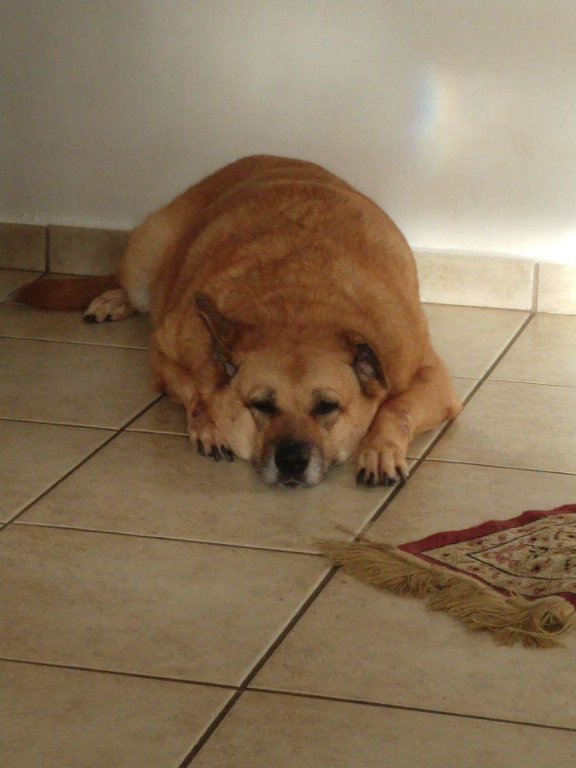
\includegraphics[width=\textwidth,keepaspectratio]{../imgs/mel.png}
                \caption{Imagem original}
            \end{subfigure}
            \begin{subfigure}{0.24\textwidth}
                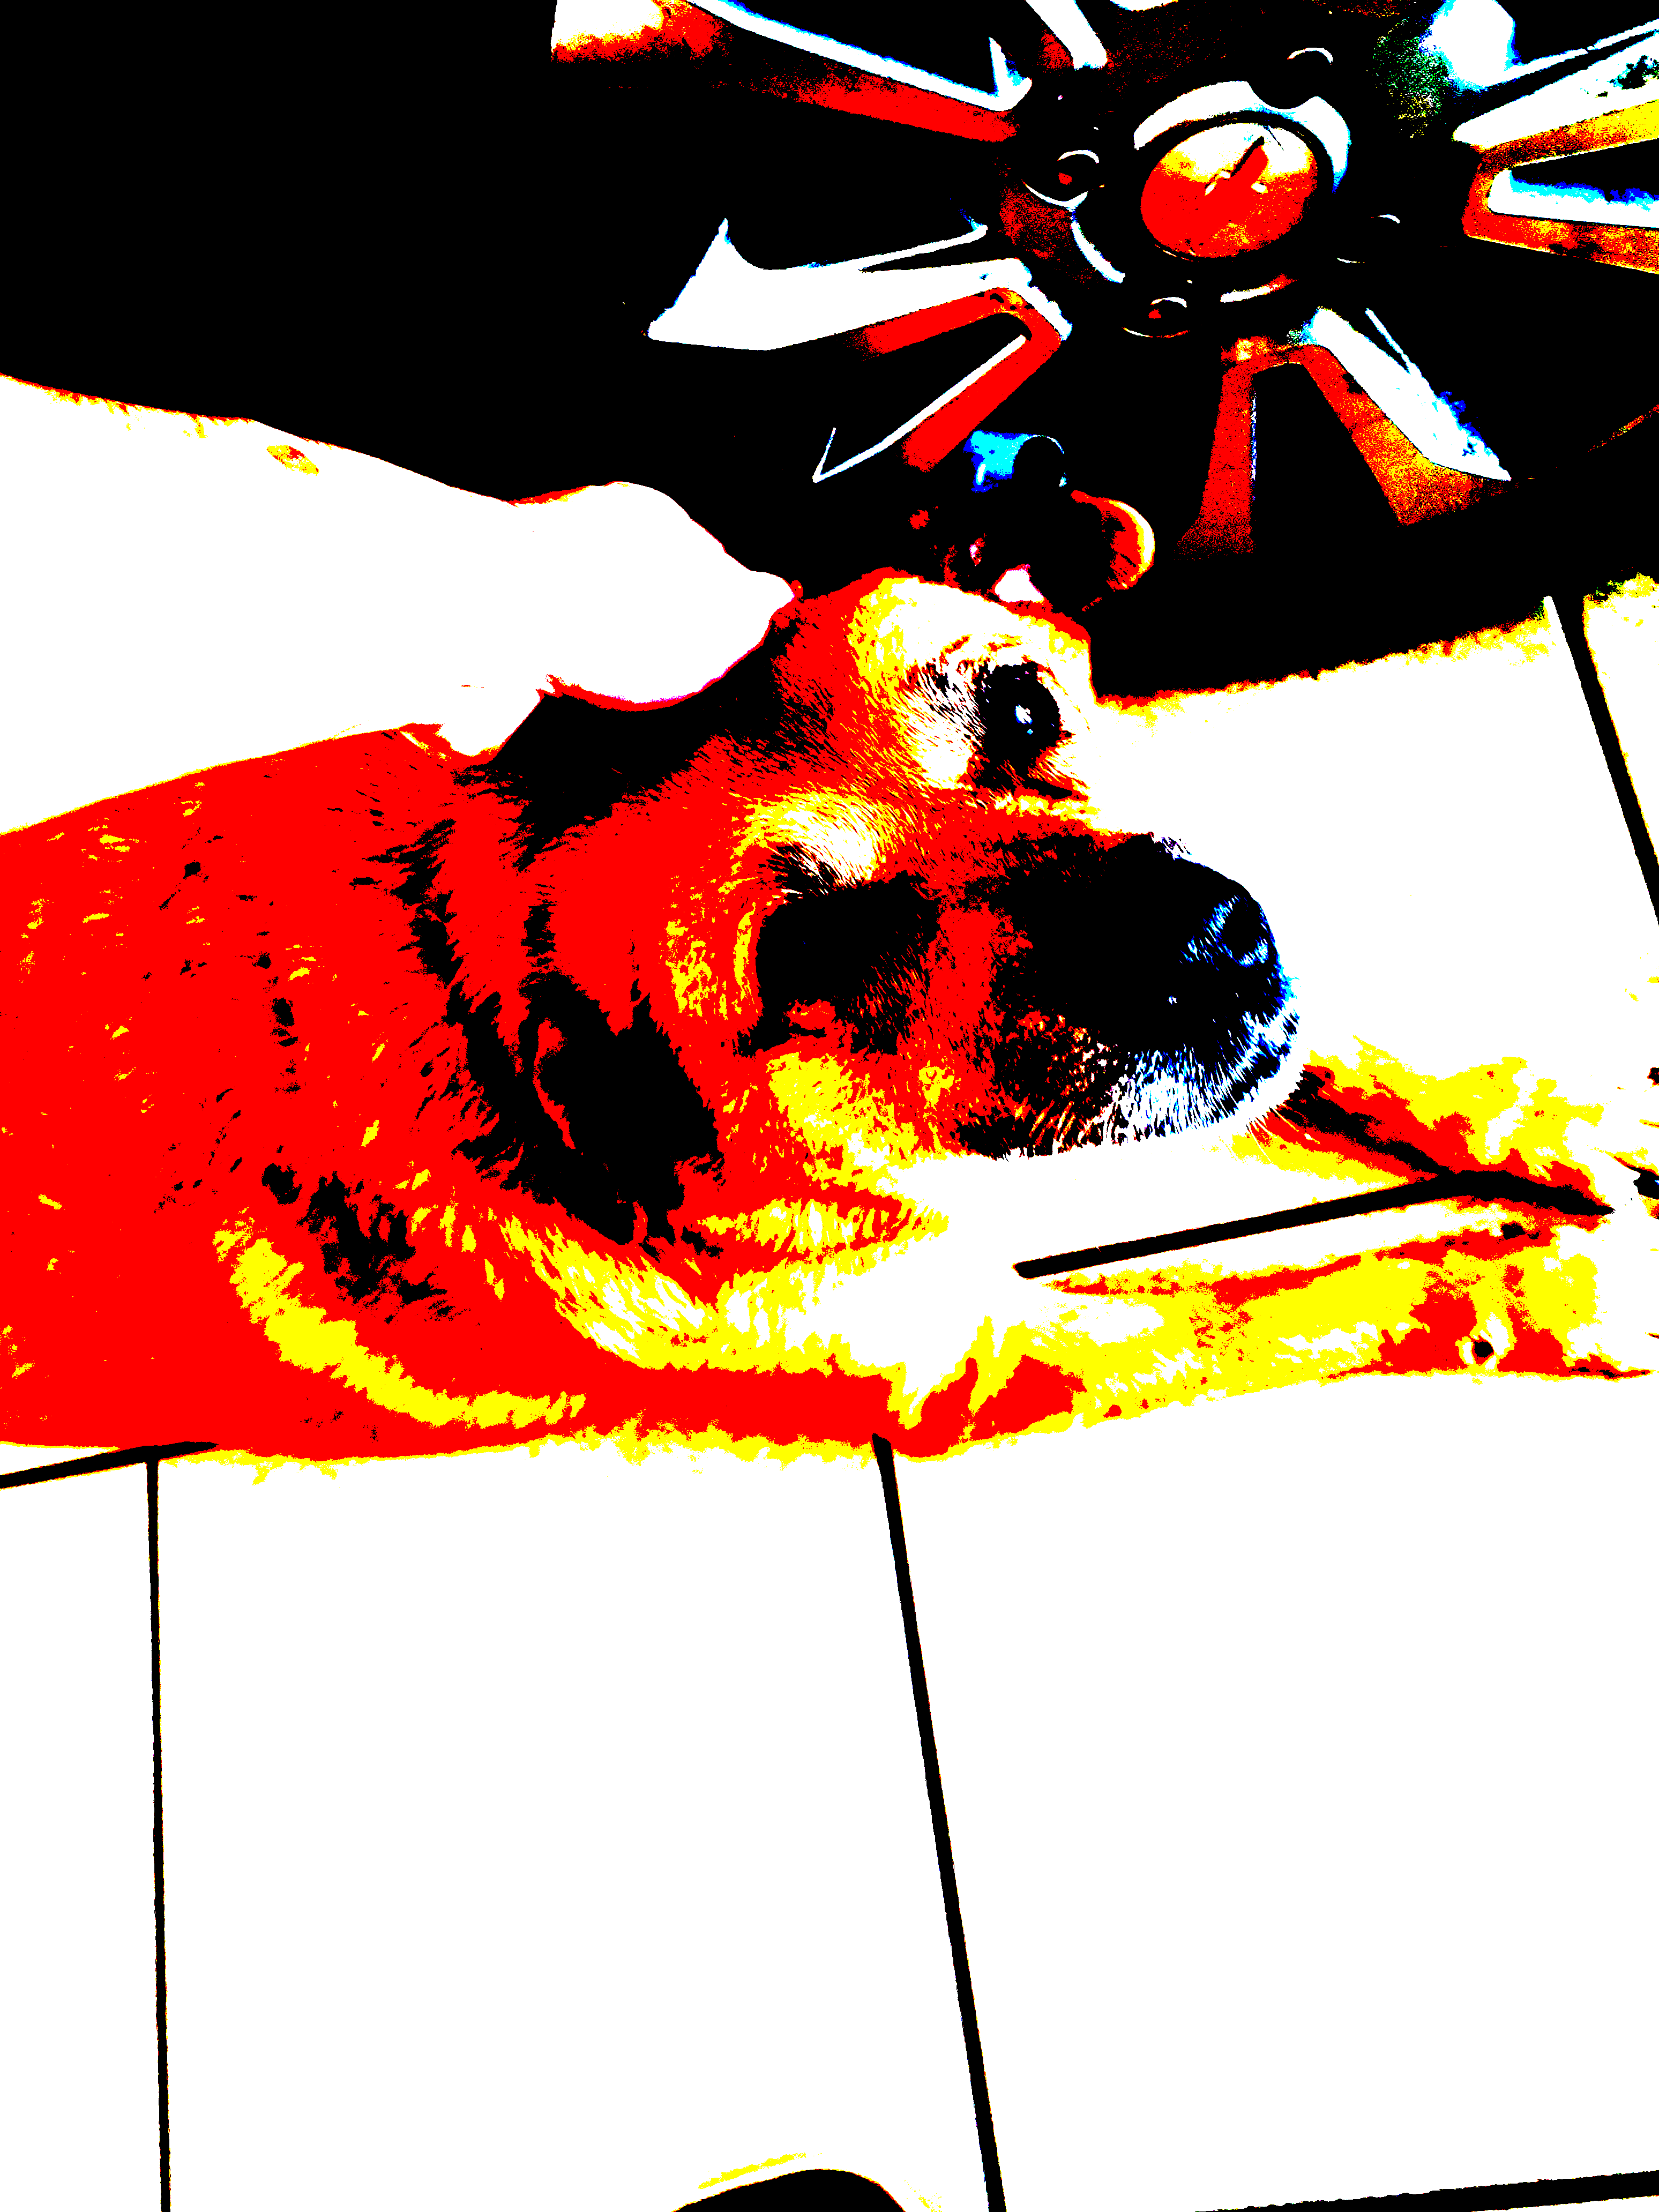
\includegraphics[width=\textwidth,keepaspectratio]{../imgs/mel-binarizada.png}
                \caption{Imagem binarizada sem difusão de erro}
            \end{subfigure}

            \caption{Comparativo para binarização sem difusão}
            \label{fig:binarizada-sem_difusao}
        \end{figure}

    \subsection{Difusão de erro de Floyd-Steinberg}

        A difusão de Floyd-Steinberg, mostrada na \cref{fig:binarizada-floyd_steinberg}, apesar de ser uma melhora considerável quando comparado com a binarização simples, apresenta um destaque grande às linhas de 45 graus.

        Essas linhas são a causa das distorções de cores acentuadas, pois a propagação das cores é muito intensa, passando o limite dos objetos, de forma a cobrir trechos em que a cor estaria mais suavizada, aumentando a sensação visual de supersaturação da imagem resultante.

        \begin{figure}
            \centering
            \begin{subfigure}{0.24\textwidth}
                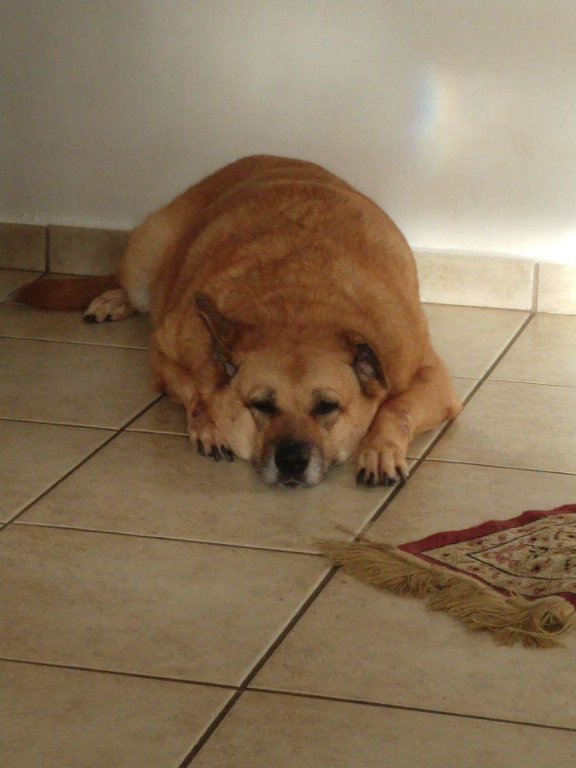
\includegraphics[width=\textwidth,keepaspectratio]{../imgs/mel.png}
                \caption{Imagem original}
            \end{subfigure}
            \begin{subfigure}{0.24\textwidth}
                \includegraphics[width=\textwidth,keepaspectratio]{../imgs/mel_binarizada-floyd_steinberg.png}
                \caption{Imagem com difusão de erro Floyd-Steinberg}
            \end{subfigure}

            \caption{Comparativo para binarização com difusão de erro de Floyd-Steinberg}
            \label{fig:binarizada-floyd_steinberg}
        \end{figure}

    \subsection{Difusão de erro de Burkes}

        A difusão de Burkes possui os mesmos problemas que as de Floyd-Steinberg, porém em menor intensidade, como podemos ver na \cref{fig:binarizada-floyd_steinberg-burkes}. Isso ainda resulta em um notável aumento na saturação aparente da imagem.

        \begin{figure}
            \centering
            \begin{subfigure}{0.24\textwidth}
                \includegraphics[width=\textwidth,keepaspectratio]{../imgs/mel_binarizada-floyd_steinberg.png}
                \caption{Imagem com difusão de erro Floyd-Steinberg}
            \end{subfigure}
            \begin{subfigure}{0.24\textwidth}
                \includegraphics[width=\textwidth,keepaspectratio]{../imgs/mel_binarizada-burkes.png}
                \caption{Imagem com difusão de erro Burkes}
            \end{subfigure}

            \caption{Comparativo entre difusão de erro de Floyd-Steinberg e Burkes}
            \label{fig:binarizada-floyd_steinberg-burkes}
        \end{figure}

        Podemos comparar ainda a intensidade das linhas à 45 graus entre as duas na \cref{fig:binarizada-floyd_steinberg-burkes-linhas}: em Floyd-Steinberg é mais acentuada e forte, já em Burkes é fina e maior, porém imita a textura. Por conta disso, a de Burkes parece mais natural quando vista a longa distância.

        \begin{figure}
            \centering
            \begin{subfigure}{0.24\textwidth}
                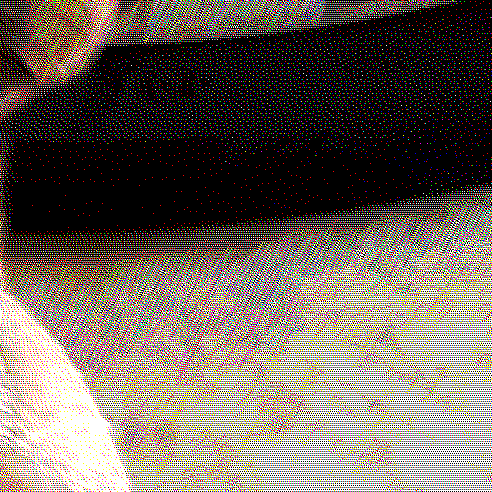
\includegraphics[width=\textwidth,keepaspectratio]{../imgs/mel_binarizada-floyd_steinberg-detalhe1.png}
                \caption{Imagem com difusão de erro Floyd-Steinberg}
            \end{subfigure}
            \begin{subfigure}{0.24\textwidth}
                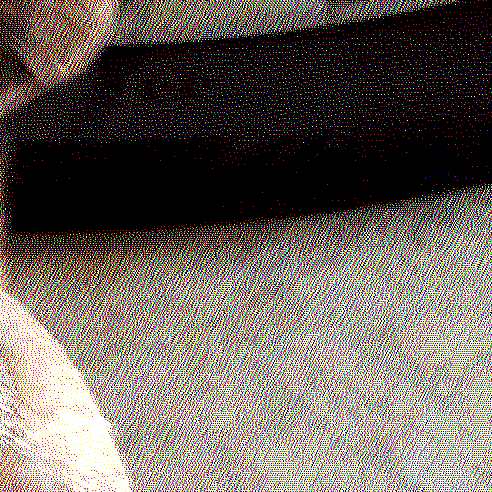
\includegraphics[width=\textwidth,keepaspectratio]{../imgs/mel_binarizada-burkes-detalhe1.png}
                \caption{Imagem com difusão de erro Burkes}
            \end{subfigure}

            \caption{Comparativo entre linhas à 45 graus em Floyd-Steinberg e Burkes}
            \label{fig:binarizada-floyd_steinberg-burkes-linhas}
        \end{figure}

    \subsection{Difusão de erro de Stevenson-Arce}

        A difusão de Stevenson-Arce mantém de forma muito eficiente a fidelidade às cores da imagem original, como visto na \cref{fig:binarizada-stevenson_arce}. Podemos notar entretanto a adição de um ruído intenso nos trechos muito claros ou escuros, causado pela presença marcante das linhas horizontais quando visualizamos de perto a imagem (\cref{fig:binarizada-stevenson_arce-destaque}).

        \begin{figure}
            \centering
            \begin{subfigure}{0.24\textwidth}
                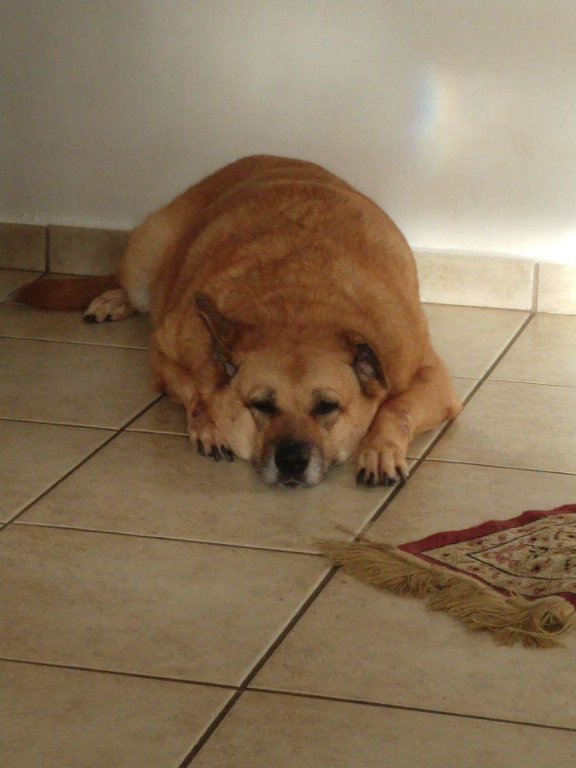
\includegraphics[width=\textwidth,keepaspectratio]{../imgs/mel.png}
                \caption{Imagem original}
            \end{subfigure}
            \begin{subfigure}{0.24\textwidth}
                \includegraphics[width=\textwidth,keepaspectratio]{../imgs/mel_binarizada-stevenson_arce.png}
                \caption{Imagem com difusão de erro Stevenson-Arce}
            \end{subfigure}

            \caption{Comparativo entre imagem original e a difusão de erro de Stevenson-Arce}
            \label{fig:binarizada-stevenson_arce}
        \end{figure}

        \begin{figure}
            \centering
            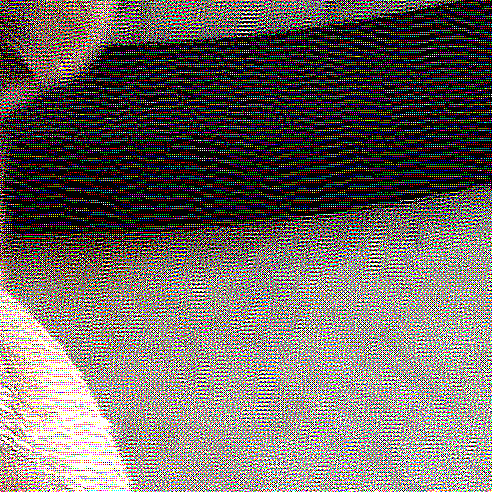
\includegraphics[width=0.45\textwidth,keepaspectratio]{../imgs/mel_binarizada-stevenson_arce-detalhe1.png}
            \caption{Destaque nas linhas horizontais de Stevenson-Arce}
            \label{fig:binarizada-stevenson_arce-destaque}
        \end{figure}


    \subsection{Difusão de erro de Jarvis-Judice-Ninke}

        Em Jarvis-Judice-Ninke, temos a presença acentuada de linhas horizontais em cores escuras e linhas a 135 graus nas claras, notável apenas a curtas distâncias (\cref{fig:binarizada-jarvis_judice_ninke-destaque}). Apesar disso, a grandes distâncias, é muito fiel à imagem original.

        \begin{figure}
            \centering
            \begin{subfigure}{0.24\textwidth}
                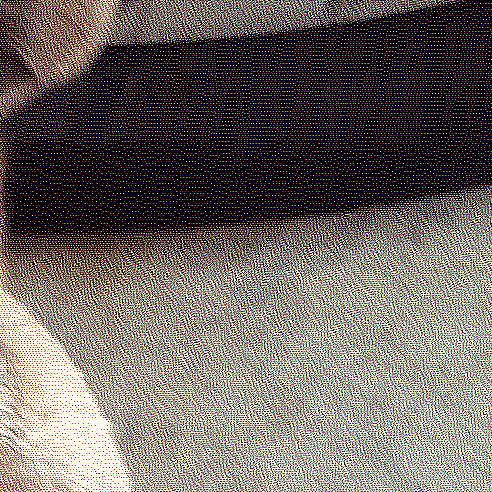
\includegraphics[width=\textwidth,keepaspectratio]{../imgs/mel_binarizada-jarvis_judice_ninke-detalhe1.png}
                \caption{Linhas horizontais em cores escuras}
            \end{subfigure}
            \begin{subfigure}{0.24\textwidth}
                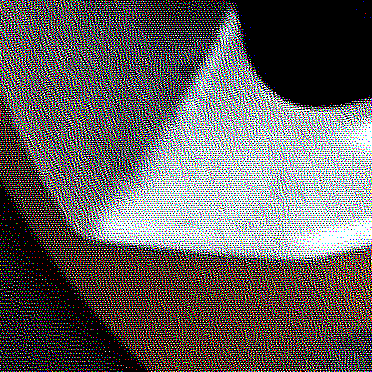
\includegraphics[width=\textwidth,keepaspectratio]{../imgs/mel_binarizada-jarvis_judice_ninke-detalhe2.png}
                \caption{Linhas a 135 graus em cores claras}
            \end{subfigure}

            \caption{Destaque a curta distância da difusão de erro de Jarvis-Judice-Ninke}
            \label{fig:binarizada-jarvis_judice_ninke-destaque}
        \end{figure}

    \subsection{Difusão de erro de Sierra}

        Como em Jarvis-Judice-Ninke, a difusão de Sierra também possui linhas a 135 graus visíveis a curtas distâncias e é bastante fiel à imagem original. A intensidade das linhas horizontais em cores escuras, no entanto, é bem menos acentuada, como podemos notar na \cref{fig:binarizada-sierra-destaque}.

        \begin{figure}
            \centering
            \begin{subfigure}{0.24\textwidth}
                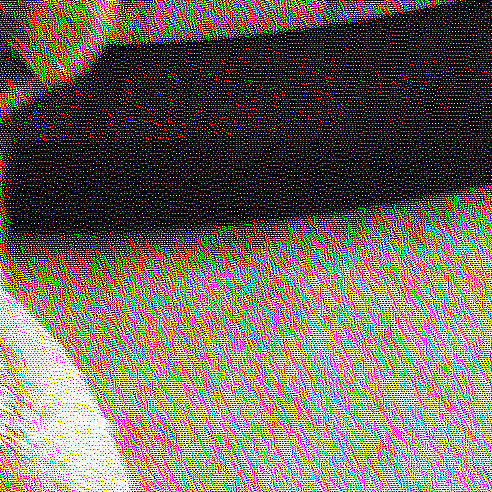
\includegraphics[width=\textwidth,keepaspectratio]{../imgs/mel_binarizada-sierra-detalhe1.png}
                \caption{Linhas horizontais em cores escuras}
            \end{subfigure}
            \begin{subfigure}{0.24\textwidth}
                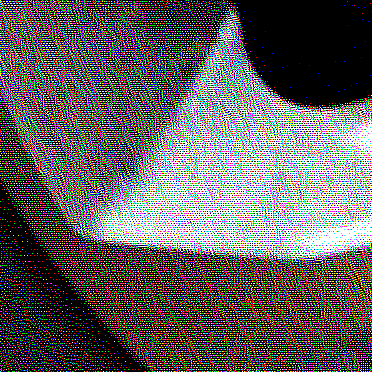
\includegraphics[width=\textwidth,keepaspectratio]{../imgs/mel_binarizada-sierra-detalhe2.png}
                \caption{Linhas a 135 graus em cores claras}
            \end{subfigure}

            \caption{Destaque a curta distância da difusão de erro de Sierra}
            \label{fig:binarizada-sierra-destaque}
        \end{figure}

    \subsection{Difusão de erro de Stucki}

        Na imagem testada, foi o melhor método de difusão de erro: é notável apenas pequenas linhas a 135 graus nas cores claras quando visto de perto. Quando visto de longe, é muito fiel e difícil identificar a imagem que foi processada.

        \begin{figure}
            \centering
            \begin{subfigure}{0.24\textwidth}
                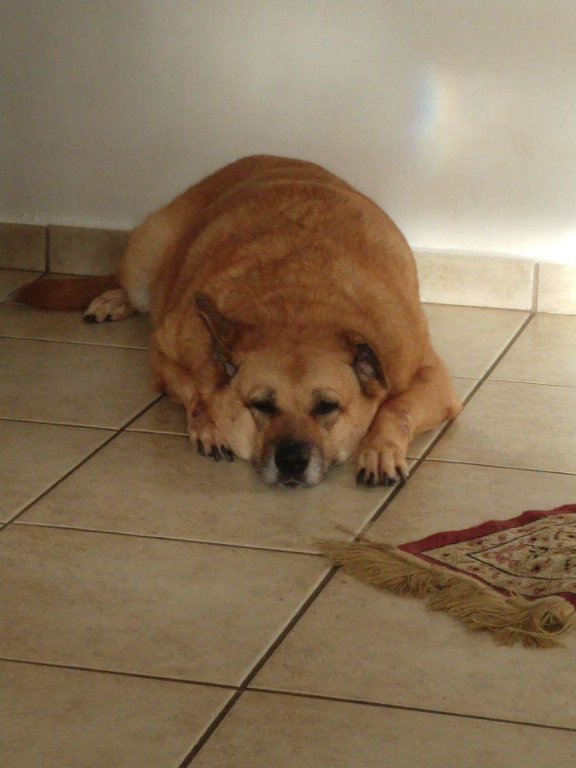
\includegraphics[width=\textwidth,keepaspectratio]{../imgs/mel.png}
                \caption{Imagem original}
            \end{subfigure}
            \begin{subfigure}{0.24\textwidth}
                \includegraphics[width=\textwidth,keepaspectratio]{../imgs/mel_binarizada-stucki.png}
                \caption{Imagem com difusão de erro Stucki}
            \end{subfigure}

            \caption{Comparativo para binarização com difusão de erro de Stucki}
            \label{fig:binarizada-stucki}
        \end{figure}

        Podemos ainda avaliar melhor as diferenças entre Sierra com Stucki nas \cref{fig:binarizada-sierra-stucki-claras,fig:binarizada-sierra-stucki-escuras}.

        \begin{figure}
            \centering
            \begin{subfigure}{0.24\textwidth}
                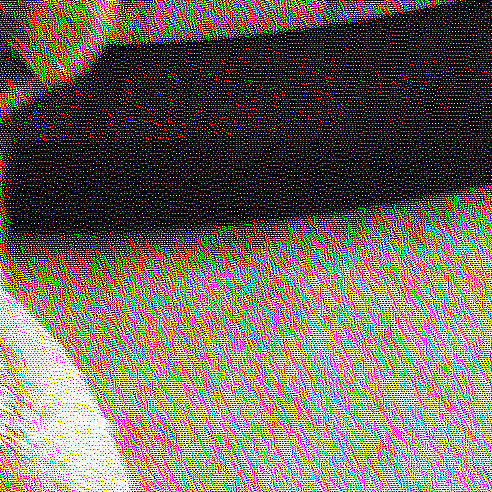
\includegraphics[width=\textwidth,keepaspectratio]{../imgs/mel_binarizada-sierra-detalhe1.png}
                \caption{Detalhe de linhas a 135 graus em Sierra}
            \end{subfigure}
            \begin{subfigure}{0.24\textwidth}
                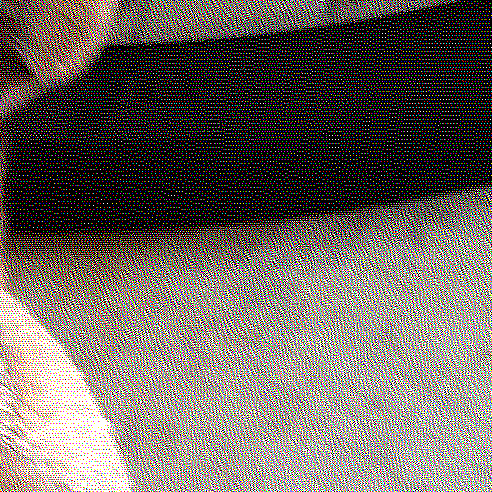
\includegraphics[width=\textwidth,keepaspectratio]{../imgs/mel_binarizada-stucki-detalhe1.png}
                \caption{Detalhe de linhas a 135 graus em Stucki}
            \end{subfigure}

            \caption{Comparativo entre linhas à 135 graus em Sierra e Stucki em cores mais claras}
            \label{fig:binarizada-sierra-stucki-claras}
        \end{figure}

        \begin{figure}
            \centering
            \begin{subfigure}{0.24\textwidth}
                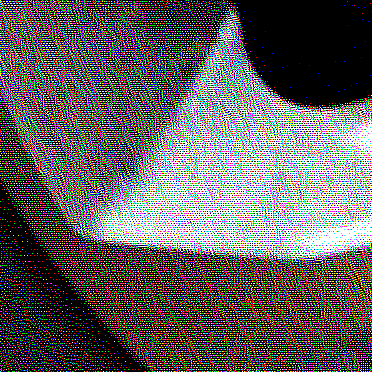
\includegraphics[width=\textwidth,keepaspectratio]{../imgs/mel_binarizada-sierra-detalhe2.png}
                \caption{Detalhe de linhas a 135 graus em Sierra}
            \end{subfigure}
            \begin{subfigure}{0.24\textwidth}
                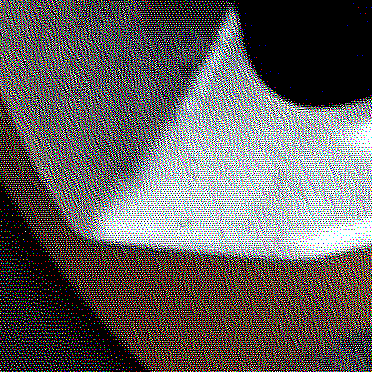
\includegraphics[width=\textwidth,keepaspectratio]{../imgs/mel_binarizada-stucki-detalhe2.png}
                \caption{Detalhe de linhas a 135 graus em Stucki}
            \end{subfigure}

            \caption{Comparativo entre linhas à 135 graus em Sierra e Stucki em cores mais escuras}
            \label{fig:binarizada-sierra-stucki-escuras}
        \end{figure}

        Na \cref{fig:binarizada-sierra-stucki-claras} podemos notar que Stucki imita melhor a textura em cores claras do que Sierra. Na \cref{fig:binarizada-sierra-stucki-escuras}, ambas possuem os mesmos riscos visíveis, porém em Sierra são mais intensos por serem maiores e às vezes fazendo uma linha contínua.


\section{Conclusão}

    Concluímos que, para a imagem colorida de grande dimensão que temos, a difusão de erro de Stucki com binarização em cada camada de cor produz resultados muito fieis a imagem original.

    Além disso, notamos como a propagação de erros pode, por um lado, auxiliar muito na fidelidade da imagem em relação à original, porém, pelo outro, adicionar artefatos muito perceptíveis, como aumentar saturação aparente, adicionar ruídos ou ainda linhas irreais e notáveis.

\end{document}
